\section{评测协议}\label{sec:protocol}

本节定义贯穿全文的评测协议。所有实验脚本共享同一套脚手架：模型单例 + 热启动状态 + teacher-forced
流式评测 + 文本源切分 + 组件手术工具。

\subsection{数据与 held-out 切分}\label{sec:data}

\textbf{语料。}预训练语料为 \texttt{pretrain.jsonl}（约 9.5\,GB，每行 \texttt{\{"text": ...\}}），
微调语料为 \texttt{sft.jsonl}（约 14\,GB，每行多轮对话）。训练按流（stream）组织：
本文检查点（v\_0d3）为 \texttt{chunk\_size}=192 条并行流，每条流对应文件的一段连续 chunk（约 49.4\,MB）。

\textbf{零污染 held-out。}训练在 step $144{,}000$ 时，每条流已消费 $144{,}000\times64\ \mathrm{B}=9.2$\,MB
（这是从训练步数与 patch 长度推算的上界）。因此本文从每条流 chunk 内\textbf{偏移 $\ge20$\,MB 处}取行，
再按 seed 洗牌拼成评测文本——取行位置远超已消费区，属同分布零污染。
\textbf{跨域档}取 \texttt{sft.jsonl} 尾部（深度按 seed 随机化）；
\textbf{消费区档}（成员推断用）取流 0 chunk 内 $[0.5,7]$\,MB 的随机偏移，
即训练确实见过的文本。$\mathrm{n}$-gram 重叠率报告的精确统计 \pending{待补：4-gram 重叠率明细见附录 \ref{app:decontam}}。

\textbf{合成档。}可打印 ASCII（字节 $\in[33,122]$，刻意 OOD）与词表内高频词对（分布内）两类，
用于前向学习与遗忘类实验（附录 \ref{app:c1}、\ref{app:g}）。

\subsection{主指标：teacher-forced bits/byte}\label{sec:metric}

\textbf{前向协议完全镜像训练前向：}patch 大小 $64$、相邻窗口重叠 1 字节
（输入 \texttt{ids[64k:64k+64]}，目标 \texttt{ids[64k+1:64k+65]}），
$\mathrm{model.eval}()$ + bf16 autocast + \texttt{inference\_mode}，不做生成式采样。
指标为 teacher-forced 交叉熵，以 \textbf{bits/byte}（$=\mathrm{nats}/\ln 2$）报告；
机会线为 $\log_2 300 \approx 8.23\ \mathrm{bit/byte}$（对 300 个字节均匀瞎猜）。

\textbf{状态流必须逐 patch 推进。}评测不能跳过任何 patch 的前向——跳过会冻结状态推进，
测出来的就不是同一条流（本文实验中都只跳过「计分」，不跳过「前向」）。

\textbf{口径说明（两处容易混淆的细节）。}
（i）当所有计分 patch 长度相同时，「每 patch 均值的均值」与「每 token 均值」严格相等，
因此 bits/byte 与逐 token 均值可以直接互换；本文实验脚本中两种实现都出现过，
所有报告数字都在等长 patch 窗口上取得，故不受该差异影响。
（ii）$\mathrm{n}$-gram 复现类指标（\S\ref{sec:b2}）的「距离」以字节计，在本模型中字节即 token。

\subsection{起点状态与实验条件声明}\label{sec:cond}

按「每次评测显式声明 \{\,起点状态,\, $\mathit{lock}$ 与否,\, 重置点\,\}」的约定，
本文所有结果表都标注这三个条件。起点状态三种来源：
\textbf{热启动}（训练稳态快照）、\textbf{空白}（恒等 memory $+$ 零 recurrent/queue/MTM）、
\textbf{热启动 $+$ 插件}（如仅回滚 \texttt{memory} 或仅清零 \texttt{recurrent}，见 \S\ref{sec:surgery}）。

\textbf{关于空白态的适用性。}空白起步使 delta 规则写读链路偏离训练操作点，
它在损失上表现为结构性失效（\S\ref{sec:a1}），因此本文\textbf{不以空白作为主表基线}，
而以热启动为基线、以「热启动 $-$ 空白」的差作为「状态贡献」的度量，
并把空白的绝对水平仅用作参照。出于同一原因，凡涉及「模型记住了训练语料吗」的问题
（\S\ref{sec:dline}），必须\textbf{双报}两种起点。

\subsection{统计口径}\label{sec:stats}

\textbf{（i）文本真随机化。}同一实验的多个 seed 必须改变\textbf{取文本的偏移}，
否则多个「seed」实际是同一段文本，会给出假窄的置信区间（本文脚手架在早期版本犯过该错并已修正）。
\textbf{（ii）成对报告。}凡是同一文本上的两条件对照（如 write vs $\mathit{lock}$），
先算每个 seed 的差值再取均值，而非分别取均值后相减——前者剔除了文本难度差异。
\textbf{（iii）置信区间。}报告 $1.96\times\mathrm{std}/\sqrt{n}$ 的 95\% 区间；$n\le2$ 时区间仅作参考。
\textbf{（iv）显存卫生。}连续执行多个短评测任务时逐次清空 CUDA 缓存分配器（否则会累积到 OOM，实测 25\,GB）。
\textbf{（v）确认性与探索性的区分。}第 \ref{sec:s1} 章的状态消融（A1--A6）与 B2 的主结论属于\textbf{确认性}实验：
成立条件在跑之前就写明（\S\ref{sec:problem}），实现缺陷订正后重跑仍成立。
而\textbf{自然重复的距离分桶}（\S\ref{sec:b2} 的表 \ref{tab:b2}）是\textbf{探索性/事后分组}：
桶边界由我们选定，不同距离上重复的是不同的 $\mathrm{n}$-gram 群体，因此该表用于描述形状而非做显著性检验。
附录 \ref{app:dline}--\ref{app:g} 的 D/E/G 三线（状态知识性质、稳定性、前向学习）
是在主结论之后追加的探索，用于解释机制，不承担主 claim。

\textbf{（vi）数字溯源。}本文每张表的每个数字都可追到实验包里的一个结果文件：
附录表 \ref{tab:config} 给出「脚本 $\leftrightarrow$ 实验」的对应关系，
结果文件命名统一为 \texttt{stage*\_results.json}（A1 为 \texttt{a1\_*\_per\_patch.json}）；
改口径即重跑、重跑即换文件，不做手工誊抄。表中未取得的数据一律标 \pending{}，不以估计值填充。

\subsection{状态手术：本文的操纵旋钮}\label{sec:surgery}

由于状态是显式、不可变的对象（\S\ref{sec:model-io}），本文可以在任意 patch 边界对状态做手术。
协议共用到五类操作（图 \ref{fig:protocol}），全部实现为「在某个 patch 前/后把状态替换为新对象」：

\begin{table}[t]
\centering
\caption{状态手术工具及其语义。所有操作都只改状态、不改权重。}
\label{tab:surgery}
\footnotesize
\begin{tabularx}{\linewidth}{@{}l X l@{}}
\toprule
操作 & 语义 & 用于 \\
\midrule
\texttt{lock\_mem} & 跨 patch 的持久写入关闭（patch 内 $v_{\mathrm{dyn}}$/因果分数仍在工作） & A2、B2、G2 \\
\texttt{reload\_hot\_memory} & 仅 \texttt{memory} 回训练稳态快照 & A5 \\
\texttt{zero\_recurrent} & 仅 \texttt{recurrent} 清零 & A5、C 线 \\
\texttt{blank\_queue\_mtm} & \texttt{queue} 清零 $+$ \texttt{MTM} 回恒等 & A5、C 线 \\
\textbf{freeze}$_{\text{子集}}$ & 每个 patch 前向后把指定分量子集恢复为前值（该分量跨 patch 不更新，patch 内照常更新） & A6、B2-freeze \\
\bottomrule
\end{tabularx}
\end{table}

\begin{figure}[H]
\centering
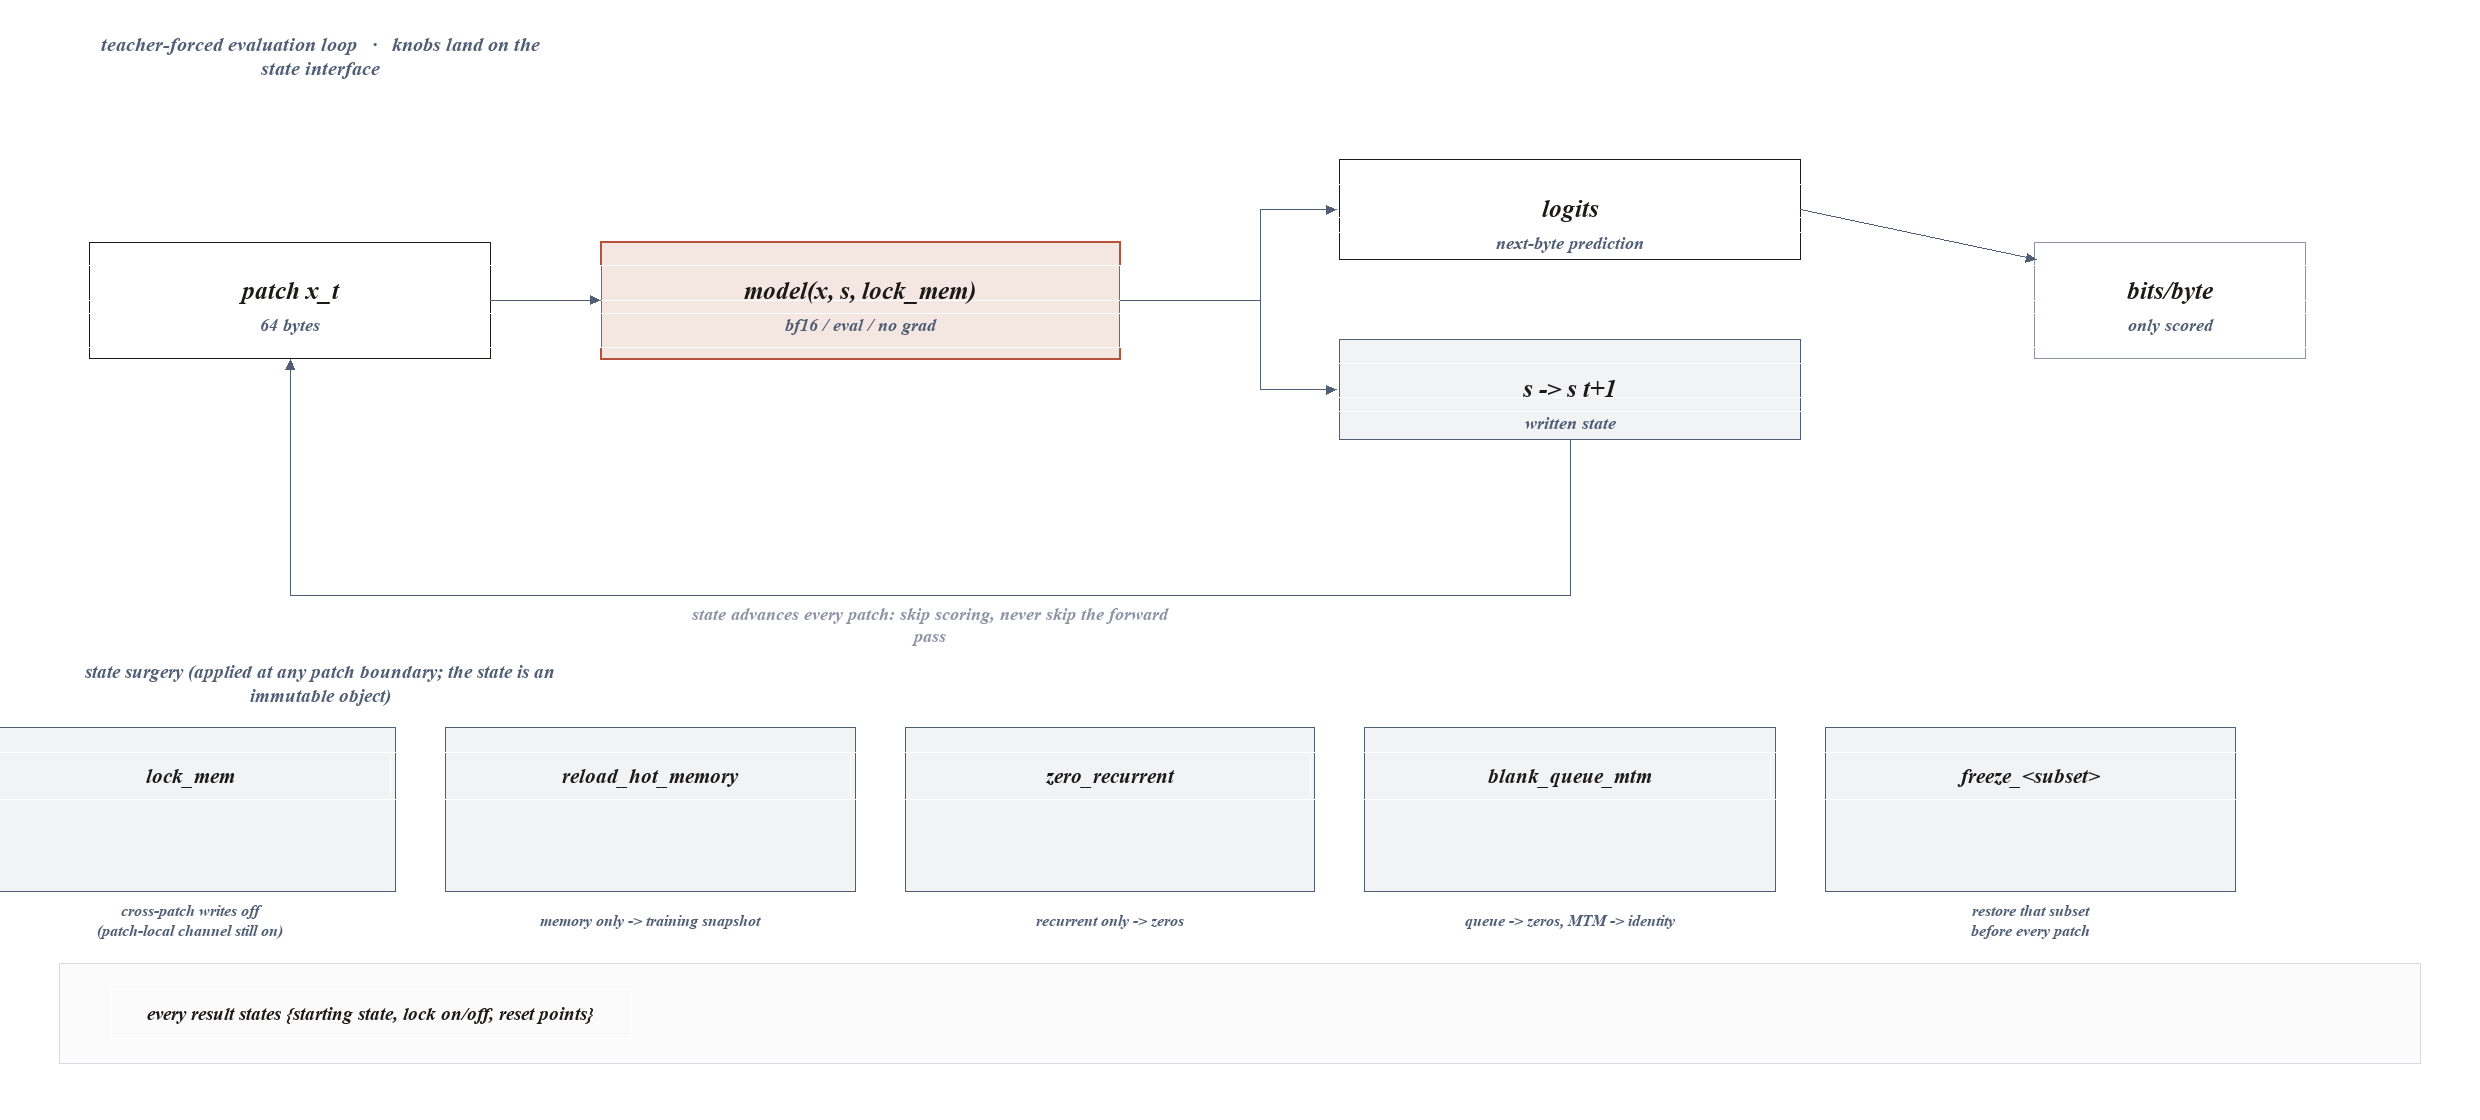
\includegraphics[width=\linewidth]{fig_protocol.png}
\caption{teacher-forced 评测回路与状态手术（Visio 绘制，源文件 \texttt{figs/fig\_protocol.vsdx}）。
每个 patch 都必须前向（跳过会冻结状态推进，只允许跳过计分）；五类手术都在 patch 边界上把状态换成新对象，
因此互不干扰的实验分支可以在同一份快照上并行开出。}
\label{fig:protocol}
\end{figure}

\textbf{$\mathit{lock}$ 与 freeze 的区别必须写清。}$\mathit{lock\_mem}$ 关闭的是\textbf{跨 patch 的持久写入}，
patch 内的动态通道仍然工作；freeze 是逐分量版本——它冻结的是某一个分量在跨 patch 尺度上的更新，
其余分量照常参与。两者互为「全局/组件」两种粒度的同一干预，
这正是 \S\ref{sec:s1-attr} 能把「写入收益」拆到组件上的原因。

\textbf{勘误与协议纪律。}本文在成稿前对实验包做了逐脚本审读，发现并订正了三处口径问题，
其中两处影响数字、一处影响结论：$\mathrm{n}$-gram 分桶的一处实现缺陷（导致「长程零衰减」的错误结论，
已修复重跑，见 \S\ref{sec:b2}）；A1 的计分窗口未对齐（已改为所有条件共用同一窗口，见 \S\ref{sec:a1}）；
受控遗忘曲线的答案位置整体偏移 66 字节（实验作废，说明见附录 \ref{app:c1}）。
这三处订正都已落到脚本里，并配了一个模型无关的位置自检脚本作为回归测试。
